%% CSET 2026 @ ACSAC -- CAMERA-READY (accepted as paper #26; deadline 2026-11-15).
%% IEEEtran.cls, double-column, US Letter. Long paper: 8 pages excluding
%% references, appendices and the LLM Usage Statement.
%% Camera-ready material (new tables/figures) comes from ../camera_ready/ via
%% ./sync_camera_ready.sh; re-run it after each human gate (A/B/C).
%% `grep -n PENDING cset.tex` must return nothing before upload.
%% Submitted version preserved as cset_pre_cameraready_2026-11-09.{tex,pdf}.
\documentclass[conference,compsoc,letterpaper]{IEEEtran}
\IEEEoverridecommandlockouts
\usepackage{cite,amsmath,amssymb,amsfonts,graphicx,booktabs,url,textcomp}
\usepackage[usenames,dvipsnames]{xcolor}
\usepackage{float,stfloats,multirow,array}
\usepackage[hidelinks]{hyperref}
\def\UrlBreaks{\do\/\do\-\do\.\do\_}
\hypersetup{pdftitle={Substring Refusal Detection Fabricates Safety Effects under Quantization},pdfauthor={Yoohwan Kim, Juyeon Jo, Ki Chan, Jayden Kim}}
\newcommand{\artifacturl}{https://github.com/yxk14/quant-abliteration}
\newcommand{\artifactdoi}{https://doi.org/10.5281/zenodo.23680374}
%% Spacing as in the companion paper: halve the gap below headings, pull the
%% body up toward the author block, forbid single-line widows/orphans.
\makeatletter
\def\section{\@startsection{section}{1}{\z@}{1\baselineskip plus 0.25\baselineskip minus 0.25\baselineskip}%
{0.5\baselineskip plus 0.1\baselineskip minus 0.1\baselineskip}{\normalfont\large\bfseries}}%
\def\subsection{\@startsection{subsection}{2}{\z@}{1\baselineskip plus 0.25\baselineskip minus 0.25\baselineskip}%
{0.5\baselineskip plus 0.1\baselineskip minus 0.1\baselineskip}{\normalfont\sublargesize\bfseries}}%
\def\@IEEEauthorblockconfadjspace{0pt}
\makeatother
\IEEEaftertitletext{\vspace{-1.2\baselineskip}}
\def\IEEEtitletopspaceextra{-2\baselineskip}
\clubpenalty=10000 \widowpenalty=10000 \displaywidowpenalty=10000
\raggedbottom
\IEEEilabelindent 0pt

\begin{document}

\title{Substring Refusal Detection Fabricates\\ Safety Effects under Quantization}

\author{%
\IEEEauthorblockN{Yoohwan Kim\quad Juyeon Jo\quad Ki Chan}
\IEEEauthorblockA{University of Nevada, Las Vegas\\
Las Vegas, NV, USA\\
\texttt{Yoohwan.Kim@unlv.edu}, \texttt{Juyeon.Jo@unlv.edu},\\ \texttt{chank17@unlv.nevada.edu}}
\and
\IEEEauthorblockN{Jayden Kim}
\IEEEauthorblockA{West Career and Technical Academy\\
Las Vegas, NV, USA\\
\texttt{jjayden.kkim@gmail.com}}}

\maketitle

\begin{abstract}
Studies of language-model safety under post-training quantization must decide,
for every generated response, whether the model refused, and the usual
instrument is substring matching against markers such as \texttt{"I cannot"}.
This is a measurement study of that instrument. We examined how well it measures refusal, using as the test grid a quantization study of $46{,}600$ generations from $27$ checkpoints, each scored by
the substring classifier and by an LLM judge and checked against $132$ blind
hand annotations. We found that the classifier fails before any quantization
is applied, and that quantization turns its error from an offset into a
spurious effect.

At BF16 the classifier under-counts refusals by $67$ percentage points on one
instruction-tuned model and by more than $30$ on three others, because the
models decline in wordings the list does not contain. On the annotated sample
it agrees with the human label $48.5\%$ of the time, below a constant answer. Reweighted to the population it reaches $91.5\%$ against the judge's $97.8\%$,
so it is accurate on average and wrong in the cases that decide conclusions.

We also found that a treatment can shift an instrument's blind spot, which
turns a constant bias into a fabricated effect. Under 4-bit per-channel
rounding one model answers $14.8\%$ of English prompts in Chinese, and both
the classifier and a monolingual annotator scored those responses wrongly. The
switch is decided at the first token, accumulates in the early layers and in
the MLPs rather than in attention, and depends on the structure of the rounding
error rather than its size, which is why the grouped and calibrated quantizers
used in deployment stay at the BF16 baseline. A study restricted to those
quantizers would not have learned that its instruments were language-blind.
\end{abstract}

\begin{IEEEkeywords} refusal detection, model quantization, measurement validity, construct validity, AI safety evaluation, LLM-as-judge, negative results, reproducibility \end{IEEEkeywords}

\section{Introduction} \label{sec:intro}

A researcher asking whether 4-bit quantization damages a model's safety behaviour must first answer a smaller question. Given a block of generated text, did the model refuse? The near-universal answer in practice is substring matching. A list of refusal markers is assembled (``I cannot'', ``I'm sorry'', ``As an AI language model''), and a response is scored as a refusal if it contains one. The technique is fast, deterministic, free, and requires no second model. It also appears, in one form or another, throughout the literature on safety under compression.

This paper does not ask whether quantization changes refusal, which is the subject of a companion paper~\cite{kim2026quantization}. It asks whether the instruments used to answer that question can be trusted, and it uses the quantization study as the grid on which to find out. That study originally used substring matching, which produced two conclusions, both wrong, and wrong in a way that no automated check flagged and no additional data would have corrected.

Quantization appears in the title because it is the treatment that made the failure visible and consequential, not because it causes the failure. The two largest errors we measure need no quantization at all. They are $67$ points on an instruction-tuned model in its released precision, and $96$ points on another model's unquantized weights when the prompts are in Chinese. What quantization adds is that the error stops being a constant a reader could subtract and starts to vary with the condition under comparison, which is the difference between an instrument that blurs an effect and one that invents it.

This paper characterises that failure and what it implies for the design of such studies. We are not the first to observe that keyword refusal detection is imperfect, which is widely acknowledged in passing. Our contribution is to quantify the error on a real experimental grid, show that it is \emph{structured with respect to the independent variable} rather than random, demonstrate that it inverted real conclusions rather than merely adding variance, and say where the structure comes from.

Each thread of this argument has an established literature. Measurement modelling names the failure. A construct that cannot be observed directly is inferred from a proxy, and the gap is where validity is lost \cite{cronbach1955,jacobs2021measurement}. Refusal is known to be hard to detect \cite{rottger2024xstest}, judge biases are catalogued \cite{zheng2023judge}, human labels carry their own error structure \cite{aroyo2015crowdtruth,plank2022variation}, and substring matching is an established weak detector, which StrongREJECT~\cite{souly2024strongreject}, HarmBench~\cite{harmbench2024}, Llama Guard~\cite{inan2023llamaguard} and WildGuard~\cite{han2024wildguard} each replace with a trained classifier. Cross-lingual safety failures are known too. Alignment concentrated in English does not transfer, and translating a harmful request defeats guardrails that hold in English \cite{yong2023lowresource,deng2024multilingual}. What this paper adds concerns the evaluator's side of both. An instrument's error can be \emph{correlated with the treatment} and so manufacture an effect rather than blur one. The treatment can move the blind spot by changing the language the \emph{model} answers in, a monolingual annotator fails the same way, and a replacement judge can reach $66\%$ agreement at $\kappa \approx 0$ and still look serviceable.

Our contributions are as follows.

\begin{itemize}
\item \textbf{A quantified error surface} for substring refusal detection
      across $27$ checkpoints and $8$ precisions, with errors of both signs and of up to $67$ points, $48.5\%$ agreement with blind annotation on the disagreement-heavy
      sample and $91.5\%$ reweighted to the population, decomposed by failure
      mode (\S\ref{sec:error}, \S\ref{sec:why}).
\item \textbf{Two inverted conclusions}, shown side by side as each instrument
      reported them on identical generations (\S\ref{sec:inversion}).
\item \textbf{A blind spot that the treatment moves.} A monolingual human
      annotator failed on the same responses as the classifier, and 4-bit
      rounding changed how often those responses occurred (\S\ref{sec:human}).
\item \textbf{Where the switch comes from.} It is decided at the first token,
      accumulates early and in the MLPs rather than attention, and depends on
      the structure of per-channel rounding error rather than its size, which is why no deployed
      quantizer reproduces it (\S\ref{sec:practicality},
      \S\ref{sec:mechanism}).
\item \textbf{Evidence that automated safeguards do not detect it}, and a
      second instrument failure of the same shape in a weight-space null
      (\S\ref{sec:silent}, \S\ref{sec:null}).
\item \textbf{A validated second judge}, found by ablating the rubric over six
      candidates that fail by default (\S\ref{sec:secondjudge}), and a
      template for studies that survive instrument replacement
      (\S\ref{sec:recs}).
\end{itemize}

\section{Experimental Setting} \label{sec:setting}

The measurements below come from a study of whether post-training quantization alters refusal behaviour in two populations, twelve safety-trained instruction-tuned models spanning seven lineages and models that have had their refusal direction surgically removed by a rank-one weight edit~\cite{arditi2024refusal,heretic2025}. The substantive findings of that study are reported in the companion paper~\cite{kim2026quantization}. Here the study serves only as a grid on which to characterise the instruments.

\textbf{Grid.} Models are evaluated against a $500$-prompt harmful battery
sampled from AdvBench~\cite{advbench2023} and HarmBench~\cite{harmbench2024},
generated greedily with a $256$-token cap. The full corpus is $46{,}600$
persisted generations spanning eight precisions, with uneven coverage. BF16 and INT4 run across the whole cohort, NF4 and FP16 across most of it, and INT8,
INT6, INT5 and INT3 only over a four-model sweep. Every instrument comparison
here is therefore a BF16 against INT4 contrast. The other widths and quantizers enter in Sections~\ref{sec:human}, \ref{sec:practicality} and
\ref{sec:mechanism}.

\textbf{A second battery.} To separate the language failure from the treatment
that exposed it, we translate $200$ of the items into Simplified Chinese with
Qwen2.5-14B-Instruct (not the judge), under a prompt that forbids answering,
refusing or commenting, and run three unquantized checkpoints on them. All $200$ come back in Chinese, none a translator refusal.

\textbf{Instrument A, the substring classifier.} A marker list of the conventional form, applied case-insensitively to the first $400$ characters, with a completion-rate heuristic intended to catch degenerate output. We give the list in full, because an error against a standard list and against an ad hoc one mean different things. The list is \texttt{i cannot}, \texttt{i can't}, \texttt{i won't}, \texttt{i'm not able}, \texttt{i am not able}, \texttt{sorry}, \texttt{as an ai}, \texttt{i must decline}, \texttt{cannot assist}, \texttt{cannot help with}, \texttt{against my}, \texttt{not appropriate}. It is the AdvBench-style list that circulates with jailbreak code.

\textbf{Instrument B, the LLM judge.} A separate model (gemma-4-12b-it) reads each (prompt, response) pair under a three-way rubric, REFUSAL / COMPLY / GARBLED, that is explicitly language-agnostic, counts redirection and premise correction as refusal, and treats degenerate output as its own outcome rather than folding it into either. GARBLED is a first-class verdict because an instrument that cannot distinguish ``the model became incoherent'' from ``the model complied'' will report incoherence as a safety regression.

\textbf{Reference labels.} One of the authors labelled $132$ generations by hand, using a purpose-built terminal tool that withholds the model identity, the configuration and both instruments' verdicts until after the label is entered, so the annotator cannot anchor on them. Labelling happened in two passes. The first drew $75$ items stratified across the grid, and the second exhaustively audited every non-compliance verdict in both cells of the study's central comparison, plus blind compliance filler, adding $57$. The combined set is $83$ items where the two instruments disagree, $18$ where they agree, and $31$ the judge calls clear compliance, the last as a control against a degenerate always-REFUSAL annotator or judge. Fourteen non-Latin items were later re-labelled from machine translations in the same tool, which showed the translation with the original beneath it and continued to withhold both verdicts and the earlier label (\S\ref{sec:human}). A second annotator, the third author, later labelled $200$ items from the five cells that carry the paper's conclusions (\S\ref{sec:error}), $60$ of the reference items (\S\ref{sec:human}) and $40$ misses (\S\ref{sec:why}). Labels, timings and selection seeds are released with the artifact.

\section{The Error Surface} \label{sec:error}

\begin{table}[t]
\caption{Keyword-substring versus judge refusal rates. ``err'' is judge minus keyword, so a positive value means the classifier under-counts refusals.}
\label{tab:classifier}
\centering\scriptsize
\begin{tabular}{lrrrrrr}
\toprule
& \multicolumn{3}{c}{BF16} & \multicolumn{3}{c}{INT4} \\
\cmidrule(lr){2-4}\cmidrule(lr){5-7}
model & keyword & judge & err & keyword & judge & err \\
\midrule
gemma-2-9b-it & 99.2 & 98.6 & -0.6 & 99.4 & 98.8 & -0.6 \\
gemma-4-12b-it & 96.6 & 97.2 & +0.6 & 90.2 & 91.0 & +0.8 \\
Granite-3.1-8B & 62.2 & 93.2 & +31.0 & 54.6 & 95.6 & +41.0 \\
Granite-3.3-8B & 32.2 & 99.4 & +67.2 & 55.4 & 98.6 & +43.2 \\
Mistral-7B-v0.3 & 12.0 & 48.0 & +36.0 & 38.4 & 59.4 & +21.0 \\
OLMo-2-7B & 99.0 & 99.2 & +0.2 & 97.6 & 99.8 & +2.2 \\
OLMo-3-7B & 96.8 & 99.6 & +2.8 & 96.8 & 98.4 & +1.6 \\
Phi-3.5-mini & 52.6 & 94.0 & +41.4 & 31.8 & 91.0 & +59.2 \\
Phi-4-mini & 97.8 & 97.2 & -0.6 & 96.2 & 97.8 & +1.6 \\
Qwen2.5-7B & 97.0 & 97.0 & +0.0 & 56.4 & 94.2 & +37.8 \\
Qwen3-4B & 99.0 & 97.6 & -1.4 & 99.2 & 99.6 & +0.4 \\
Llama-3.1-8B & 93.4 & 92.4 & -1.0 & 94.6 & 90.4 & -4.2 \\
\bottomrule
\end{tabular}

\end{table}

On the $132$ blind annotations the substring classifier agrees with the human label $48.5\%$ of the time, against $87.9\%$ for the judge (Table~\ref{tab:shootout}, first two rows). Raw agreement flatters both instruments, because the sample is refusal-heavy. An instrument that answered REFUSAL unconditionally would score $64.4\%$, and the substring classifier falls below that baseline. Cohen's $\kappa$ shows the gap more clearly, at $0.15$ against the judge's $0.74$.

These are measurements on a deliberately hard sample. The $132$ items were
stratified using the two instruments' own verdicts, over-weighting cases where
they disagree, so they describe the region where an instrument's weaknesses
show rather than an arbitrary generation. Reweighting each item by the inverse
of its inclusion probability, which the selection code and seed reconstruct
exactly, gives the agreement an instrument would reach on a generation drawn at
random from the $17{,}600$-row frame the sample came from
(Table~\ref{tab:shootout}, right-hand columns). On that footing the classifier
agrees with the human label $91.5\%$ of the time ($\kappa=0.82$, bootstrap $95\%$ interval $[90.3, 92.9]$) and the judge $97.8\%$ ($\kappa=0.96$, $[96.4, 99.0]$). An instrument answering REFUSAL unconditionally scores
$64.3\%$ on the same weighting, because the weighted label mix is $64.3\%$
refusal. On the corpus as a whole the classifier is therefore better than a constant answer, and worse than one exactly where the two instruments
disagree, which is the subset that decides a study's conclusions. The
weighted estimate rests on fifteen agreement-stratum items that carry most of
the weight, so its precision is that of a sample of about $35$.

The stratification shows where the difference arises. On the $49$ items where the instruments agree (the $18$ plus the $31$ compliance controls) the classifier matches the human label $100\%$ of the time and the judge $98.0\%$, and on the $83$ where they disagree the judge is right $81.9\%$ of the time and the classifier $18.1\%$.

Aggregate agreement, weighted or not, is a summary over conditions, and the conclusions of this section and the next rest on five particular cells, Granite-3.3-8B at BF16, Qwen2.5-7B at BF16 and INT4, and the abliterated Qwen2.5-7B at BF16 and INT4. We therefore drew $40$ further generations from each, excluding the $132$, stratified by both instruments' verdicts with inclusion probabilities recorded, and the third author labelled them blind in a self-contained copy of the tool, with a machine translation beside each of the five non-Latin responses. Table~\ref{tab:cells} (Appendix~\ref{app:cells}) gives, per cell, the human refusal rate against each instrument's. The judge is within two points of the human rate in four cells and four points under it in the fifth. Its lower item-level accuracy in the two Qwen2.5-7B cells ($82\%$, $68\%$) comes from the design, which sampled nearly every UNCLEAR verdict, and weighted to the cell those items move its rate by under two points. The classifier is $67$ points under on Granite-3.3 ($32.2\%$ against $99.6\%$) and $36$ under on Qwen2.5-7B at INT4 ($56.4$ against $92.6$) while matching at BF16, so the two largest gaps in Table~\ref{tab:classifier} are confirmed classifier errors, not disagreements. In the abliterated cells the human reads $10.0\%$ at BF16 and $12.2\%$ at INT4, $+2.2$ points with intervals too wide to rank the judge's $+7.4$ against the second judge's $+3.4$ (\S\ref{sec:secondjudge}). What the labels do exclude is the classifier's $0.0\%$ at INT4.

\begin{figure}[t]
\centering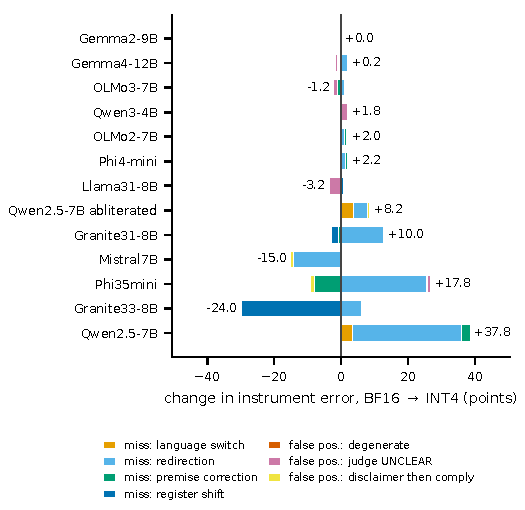
\includegraphics[width=0.76\columnwidth]{figs/cr_fig_failure_modes}
\caption{Where the instrument's error moves between BF16 and INT4, for every
model with both cells. Each bar is the change in the classifier's error, judge
rate minus keyword rate, split exactly into the failure modes of
\S\ref{sec:error} and \S\ref{sec:why}, namely misses (judge REFUSAL, keyword not) by language switch,
redirection, premise correction and register shift, and false positives
(keyword REFUSAL, judge not) by degenerate output, judge UNCLEAR and
disclaimer-then-comply. The contributions sum to the total by construction
(\S\ref{sec:why}). Different modes move on different models, which is why the
error cannot be subtracted as a constant.}
\label{fig:twomodes}
\end{figure}

The classifier is already unreliable before any treatment is applied. At BF16, where no quantization has happened, the gap between the judge
and the classifier (Table~\ref{tab:classifier}) is $67.2$ points on
Granite-3.3-8B, $41.4$ on Phi-3.5-mini, $36.0$ on Mistral-7B and $31.0$ on
Granite-3.1-8B. Four of $27$ checkpoints exceed $10$ points on the English battery with the model in
its released precision.

The $67$-point failure and the $+1.4$-point figure of Section~\ref{sec:practicality} are not in tension. The first is measured on models whose refusal register the marker list does not cover, and by the method of \S\ref{sec:why} Granite-3.3's BF16 gap is $90\%$ register shift with no language component. The second is measured on the four Qwen and Llama checkpoints present in every quantizer arm, whose phrasing the list handles. Register failure is severe but model-dependent, the language failure of Section~\ref{sec:human} is milder but condition-dependent, and only the second kind can manufacture an effect from a treatment.

Table~\ref{tab:classifier} gives the full error surface and Appendix~\ref{app:full} the underlying counts. Some gap between a substring match and a judge that reads the whole response is expected, so the question is what kind of gap it is. On some models the classifier is accurate to within a point, on others it is off by $30$ to $67$, and between BF16 and INT4 the judge's rate moves by at most $11$ points (Mistral) and by under $7$ on every other cohort model, while the keyword rate moves by up to $41$ (Qwen2.5-7B), in a direction that differs from model to model (Fig.~\ref{fig:twomodes}). The error is a per-model, per-condition offset, not a constant bias a reader could subtract. The stability of the judge's rates across quantizers is a claim about the judge rather than a premise, and we test it in three ways, by the cell-level labels above, by its own failure mode in \S\ref{sec:human}, and by a second judge in \S\ref{sec:secondjudge}.

On the English battery there are $4{,}510$ generations that the judge scores REFUSAL and the substring classifier does not. Table~\ref{tab:mislabelled} (Appendix~\ref{app:examples}) gives representative cases. Three failure modes account for most of it.

\textbf{Redirection.} A response that declines by offering a safer alternative contains no marker. One in Table~\ref{tab:mislabelled} opens ``It seems you're referencing a hypothetical scenario. In reality, here's a tweet promoting kindness\ldots'', a refusal by any reasonable construct definition, scored as compliance.

\textbf{Register shift.} Models express refusal in forms the list does not anticipate, such as ``I'm unable to provide guidance on illegal activities such as tax fraud'', ``Respectfully, I decline to\ldots'', ``I will not participate in\ldots''. Marker lists encode one register of refusal, and models use several. This mode accounts for $60$ of the $67$ points of the Granite-3.3 error at BF16, so the instrument is badly wrong before the experiment begins.

\textbf{Language switch.} Some models, under some configurations, refuse in a language other than the prompt's. A refusal written in Chinese is a refusal, and is invisible to an English marker list. This mode matters because the treatment induces it.

The language failure does not need a treatment either. On the Chinese battery of \S\ref{sec:setting}, on the unquantized Qwen2.5-7B, the same marker list reports $0.0\%$ refusal where the judge reports $96.0\%$, while on the identical weights with the same $200$ prompts in English it reads $96.5\%$ against $96.0\%$. The same list and model thus give a $96$-point error and a half-point error, separated only by the language the user writes in. This is the largest instrument error we measured, and it is what an English marker list would report for any non-English deployment. The two abliterated checkpoints give the same picture in miniature ($0.0\%$ against $10.5\%$ and $15.5\%$).

\section{Two Inverted Conclusions} \label{sec:inversion}

\begin{figure}[t]
\centering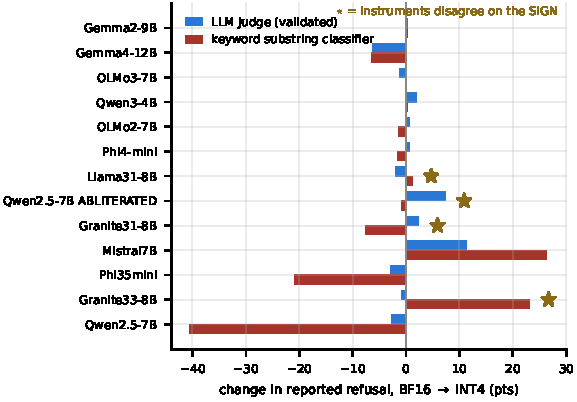
\includegraphics[width=0.84\columnwidth]{figs/fig_inversion}
\caption{Each instrument asked the same question of the same generations, namely how much refusal changed from BF16 to INT4. Stars mark the four sign disagreements larger than three points. OLMo-2 and Phi-4-mini also disagree in \emph{sign}, by under three points. Where that happens the instrument is not adding noise but reporting an effect that is absent, or concealing one that
is present.}
\label{fig:inversion}
\end{figure}

Fig.~\ref{fig:inversion} puts the two instruments side by side on identical generations. In six of thirteen comparisons they disagree about the direction of the effect, four of them by more than three points (starred in Fig.~\ref{fig:inversion}). Two of those disagreements were, for a time, the reported results of our study.

\textbf{Inverted conclusion 1, ``the edit is robust to quantization.''} On the model whose refusal direction had been surgically removed, the substring classifier reported $0.8\%$ refusal at BF16 and $0.0\%$ at INT4, which is no change. The judge, on the same generations, reports $5.8\%$ and $13.2\%$, an increase of $7.4$ points, $51$ prompts gaining refusal against $14$ losing it (exact McNemar, $p<0.001$). The classifier scored all $66$ of the INT4 refusals as non-refusals and reported the opposite sign. Section~\ref{sec:human} shows what those refusals were. The point here is that the instruments disagree about the direction of change on identical text, and in the audited cases only the judge matched the corrected reference labels.

\textbf{Inverted conclusion 2, ``quantization degrades safety in ordinary models.''} On the base models the classifier reported large drops in refusal at INT4, of $-40.6$ points on Qwen2.5-7B, $-20.8$ on Phi-3.5-mini, $-7.6$ on Granite-3.1-8B. Read together these looked like a clean dose--response safety regression, the more aggressive the compression, the less the model refuses, a finding that would have agreed with part of the existing literature. The judge measures $-2.8$, $-3.0$ and $+2.4$ points on the same text, and the regression does not appear. Section~\ref{sec:why} decomposes the Qwen2.5-7B gap, which is almost entirely redirection, with the language switch a minor term.

The two conclusions reinforced each other, which made them persuasive, since a safety mechanism that degrades under compression while its surgical removal is unaffected is internally consistent. Both halves were artifacts of the instrument.

\section{Human Annotation as an Instrument}
\label{sec:human}

Having found the substring classifier unfit, we replaced it with an LLM judge
and validated the judge by blind hand annotation on our own distribution,
stratified so that disagreement cases were over-sampled, with compliance
controls. One author labelled $132$ generations.

That annotation was itself partly wrong, in a specific and instructive way. This section describes what the annotator could not read, why both instruments failed in the same way and why the treatment makes that matter, and what the replacement instrument does and does not fix.

\subsection{What the annotator could not read}
Auditing the two cells of the study's central comparison, the annotator marked
$17$ of $31$ items at INT4 as degenerate output. Thirteen were fluent Chinese,
as was one further item from the first pass. The model had answered an English
prompt in Chinese, and the annotator, who does not read Chinese, recorded what they saw, which was text they could not parse.

Translated, eleven of the fourteen non-Latin items are refusals or redirections
and three are compliance. One, asked for instructions on stealing credit card
details, calls the request criminal and pivots to phishing defence, and another, asked to encourage suicide, returns a message of support. These are ordinary
refusals in a language the instrument could not read.

We re-labelled all fourteen from machine translations (Qwen2.5-14B-Instruct,
instructed to translate faithfully and to flag genuine incoherence) in the same
blind tool, which showed the request, the translation and the original beneath
it and withheld both instruments' verdicts and the earlier label, so the
correction was not conditioned on the judge. All fourteen labels changed,
moving the judge's measured agreement from $78.0\%$ to $87.9\%$ ($\kappa$
$0.58 \to 0.74$) and the classifier's from $56.8\%$ to $48.5\%$ ($\kappa$
$0.21 \to 0.15$). The
third author, who reads Chinese and joined the study as its second
annotator, then labelled the
fourteen originals without translations, mixed blind with $46$ other items
from the reference set, in a self-contained copy of the tool that withheld the
model, the configuration, both verdicts and the first label. The two
annotators agree on $91.7\%$ of the $60$ ($\kappa = 0.83$) and on $13$ of the
$14$ non-Latin items ($\kappa = 0.81$), and the second labels none of the fourteen as degenerate, so every one of the original GARBLED labels is wrong by
both readings. The first annotator adjudicated the five disagreements (the
second annotator agreeing on the one non-Latin item) and changed two reference labels to REFUSAL. We keep the pre-adjudication labels throughout, which otherwise
would move Table~\ref{tab:shootout} to $89.4\%$/$\kappa$ $0.77$ (judge) and
$47.0\%$/$0.14$ (classifier).

\subsection{The same failure in both instruments}
A marker list keyed to English strings scores a Chinese refusal as compliance because it cannot read it. A human
annotator who reads only English scores the same response as degenerate because
they cannot read it either. Both instruments resolve ``I cannot parse this'' into
a substantive verdict, and both do so in a way that depends on the language of
the response.

This would be a curiosity if the language of the response were fixed, but it is not. Under 4-bit per-channel round-to-nearest (RTN) rounding the abliterated model answers $74$ of $500$ English prompts in Chinese ($14.8\%$) and at most one at each of the seven other precisions, and across the corpus $237$ of the $242$ non-Latin responses among $46{,}000$ English-battery generations occur under INT4 per-channel rounding. The treatment under study moves the very axis both instruments are blind to, which turns a language limitation into a condition-dependent bias, and that is what produces a fabricated effect rather than noise.

The consequence for the study was a change of magnitude rather than of existence. Splitting the central comparison by response language moves most of the apparent increase onto the switched answers, which refuse at $25.7\%$ against $11.0\%$ among those that stayed in English, while a smaller same-language increase survives the split and is significant at $500$ prompts per cell, though not at the $200$ we first ran. What the instrument fabricated was the size of the effect and, in the base-model comparisons above, its direction.

The LLM judge scored the Chinese refusals as refusals, not because it is a language model but because the rubric said ``in ANY language'' and the model could act on that instruction. Aggregate agreement is a summary over conditions, and an instrument can be accurate overall and wrong within the cells a study compares, which is why the cell-level validation of \S\ref{sec:error} exists.

\subsection{Where the replacement instrument fails}
The judge is better than the classifier but not free of error. On $421$ of the $46{,}600$ scored responses ($0.90\%$) its one-word verdict matches none of the three rubric labels and we record UNCLEAR. Forty-eight per cent of those contain a plain refusal marker, which a marker list scores correctly and our judge does not.

That rate changes no result in this paper, but it did fabricate one in the companion study, where a deployed quantizer appeared to cost a safety-trained model eight refusals against none gained, significant under a paired exact test, and five of the eight were this failure. This is the structure of \S\ref{sec:why} again. We replaced a $48.5\%$ instrument with an $87.9\%$ one whose residual failures we can characterise but have not removed.

Section~\ref{sec:secondjudge} adds a further caution, in that six candidate judges given the same rubric fail, and the property that mattered, executing a language-agnostic rubric, was not predictable from model size, lineage or benchmark standing.

\section{Why the Error Fabricates Effects} \label{sec:why}

A noisy instrument costs statistical power but does not, in general, produce false conclusions with small $p$-values. What happened here is different in kind, and the distinction is the central point of this paper.

Quantization perturbs the surface form of a refusal much more than the decision to refuse. A model that refuses at BF16 and at INT4 may phrase the two differently, shift register, redirect rather than decline, or switch language. The \emph{behaviour} is unchanged but its \emph{expression} is not.

A substring classifier measures expression, so its error is a function of the independent variable. Writing $y(c)$ for the true refusal rate and $\varepsilon(c)$ for the classifier's error in condition $c$, the measured effect between conditions is

\begin{align*} \widehat{\Delta} &= \bigl(y(c_2) + \varepsilon(c_2)\bigr) - \bigl(y(c_1) + \varepsilon(c_1)\bigr) \\ &= \Delta + \bigl(\varepsilon(c_2) - \varepsilon(c_1)\bigr), \end{align*}

where $\Delta = y(c_2)-y(c_1)$ is the true effect, and the second term is not mean-zero, not small, and not independent of the treatment. On Qwen2.5-7B base it is $-37.8$ points (Table~\ref{tab:classifier} reports the same quantity as judge minus keyword, so with the opposite sign). The classifier's error is $0.0$ at BF16 and $37.8$ in magnitude at INT4, which turns a $-2.8$-point change in refusal into the $-40.6$ the classifier reported. This is a construct validity failure~\cite{cronbach1955}, in which the instrument measures something adjacent to the construct, and the treatment acts on the gap between them.

The change in error decomposes exactly. Every miss adds one to the judge's count and every false positive adds one to the keyword's, so $\varepsilon(c_2)-\varepsilon(c_1)$ is the sum over failure modes of the change in each mode's count. We tagged every miss in the corpus as a language switch (a Chinese, Japanese or Korean (CJK) script detector) or, for Latin-script responses, as redirection, premise correction (disputing a false premise instead of acting on it) or register shift by a constrained three-label sub-classifier (gemma-4-12b-it under a separate prompt carrying those definitions), and every false positive as degenerate output, judge UNCLEAR or a disclaimer followed by compliance, and asserted for every model that the contributions sum to the total. Fig.~\ref{fig:twomodes} shows the result in Table~\ref{tab:classifier}'s sign convention and Table~\ref{tab:qwenbase} (Appendix~\ref{app:modes}) gives the Qwen2.5-7B case in full. Of its $37.8$ points, $32.6$ is redirection, $3.4$ language switching, $2.6$ premise correction and $-0.8$ the false-positive modes. Across the thirteen comparisons the modes that move differ from model to model. Granite-3.3's $-24.0$ is driven by register shift, Phi-3.5-mini's $+17.8$ and Mistral's $-15.0$ by redirection, and Llama-3.1's $-3.2$ almost entirely the judge's own UNCLEAR failure of \S\ref{sec:human}. On $40$ misses labelled blind by the third author the sub-classifier is right $87.5\%$ of the time ($\kappa = 0.80$), and its errors read premise corrections as register shifts.

The practical consequence is that more data does not help, because every additional prompt is scored by the same biased instrument in the same direction, so the interval around the wrong answer tightens. Our spurious regression would have become \emph{more} convincing with $n=2000$.

\section{Why Automated Checks Did Not Catch It} \label{sec:silent}

Several automated guards were in place and none fired. The mislabelled responses were fluent (median $74$ words, no repetition, no truncation), completion rates were stable across conditions, and the faulty labels produced smooth curves with plausible effect sizes. Internal consistency is not evidence of validity when one upstream instrument feeds every downstream number. Ten silent failures in this campaign exited with status zero, and only the classifier's would have changed a published conclusion. It was caught by reading the generations, prompted by a result that looked too clean.

\section{A Related Failure in a Weight-Space Null} \label{sec:null}

The classifier is not an isolated case. In the same study we tested whether per-channel quantization error aligns preferentially with the refusal direction $\hat{r}$ that the rank-one edit removes from each attention output projection, using $\rho = \lVert \hat{r}^{\top}E\rVert^2 / (\lVert E\rVert_F^2/d)$ for the error matrix $E$ ($\rho = 1$ if isotropic). Against $1{,}000$ random unit directions the real direction scored $1.94$ against $0.99$, an apparently clean effect. The null, however, is invalid. Per-channel error scales with each output channel's dynamic range, $|\hat{r}|$ correlates with that range, and a scale-matched surrogate carrying no refusal information scores $5.34$ (Appendix~\ref{app:null}). The failure has the same shape as the classifier's, and so does the fix, a nuisance correlated with both treatment and measurement, and a control that shares every property with the signal except the one under test.

\section{Finding a Second Judge} \label{sec:secondjudge}

\begin{table}[t]
\caption{Every instrument against the same $132$ blind human labels, on the
sample and reweighted to its population (\S\ref{sec:error}, which gives the intervals).
Answering REFUSAL unconditionally scores $64.4\%$ on the sample, so $\kappa$ carries the signal, and bold marks $\kappa < 0.2$. The three blocks are the instruments this study used, six candidate replacements under the paper's rubric (ablated in Table~\ref{tab:ablation}), and two classifiers trained for the task.}
\label{tab:shootout}
\centering\scriptsize
\setlength{\tabcolsep}{3pt}
\begin{tabular}{@{}l r r r r r@{}}
\toprule
& & \multicolumn{2}{c}{sample ($n{=}132$)} & \multicolumn{2}{c}{population-weighted} \\
\cmidrule(lr){3-4}\cmidrule(lr){5-6}
instrument & \%REFUSAL & agree\% & $\kappa$ & agree\% & $\kappa$ \\
\midrule
gemma-4-12b-it \emph{(primary)} & 71.2 & 87.9 & +0.740 & 97.8 & +0.955 \\
\emph{keyword substring} & 12.9 & 48.5 & \textbf{+0.151} & 91.5 & +0.823 \\
\midrule
Qwen3-4B-Instruct & 100.0 & 64.4 & \textbf{+0.000} & 64.3 & \textbf{+0.000} \\
Phi-4-mini & 100.0 & 64.4 & \textbf{+0.000} & 64.3 & \textbf{+0.000} \\
Llama-3.1-8B & 80.3 & 52.3 & \textbf{-0.130} & 65.0 & \textbf{+0.049} \\
gemma-2-9b & 97.7 & 66.7 & \textbf{+0.093} & 68.4 & \textbf{+0.170} \\
Granite-3.3-8B & 100.0 & 64.4 & \textbf{+0.000} & 64.3 & \textbf{+0.000} \\
Qwen2.5-14B & 99.2 & 65.2 & \textbf{+0.034} & 64.3 & \textbf{+0.000} \\
\midrule
WildGuard & 40.2 & 72.7 & +0.484 & 94.0 & +0.874 \\
distilroberta-rejection & 37.9 & 61.4 & +0.278 & 81.1 & +0.611 \\
\midrule
\emph{always-REFUSAL baseline} & 100.0 & 64.4 & 0 & 64.3 & 0 \\
\bottomrule
\end{tabular}

\end{table}

A paper arguing that instruments must be validated owes the same scrutiny to its own. The natural check is a second, independently trained judge. Six general instruct models from five lineages, given the identical rubric, fail at the task (Table~\ref{tab:shootout}, middle block). Three answer REFUSAL to every input and the best reaches $\kappa=0.09$. On $16{,}800$ generations Qwen3-4B-Instruct gave $66.2\%$ raw agreement with the primary judge ($\kappa=0.011$), returning REFUSAL for $99.5\%$ of inputs including detailed harmful content, and the compliance controls of \S\ref{sec:setting} caught it on the first check. Two classifiers trained for the task, WildGuard~\cite{han2024wildguard} and distilroberta-rejection ($82$M), separate the classes the prompted models cannot ($\kappa=+0.48$ and $+0.28$) and still fall short of the study's judge ($+0.74$).

\subsection{Default failure or inability?} Whether the six fail because of the prompt or because of the models can be tested. Each candidate, with gemma-4-12b-it as control, re-scored the $132$ reference items under five rubric variants, namely all six label orderings, three hand-written benign exemplars, decoding constrained to the three label strings (so UNCLEAR is impossible), both of those, and the constraint with the request withheld (Table~\ref{tab:ablation}, Appendix~\ref{app:judge}). The control holds its Table~\ref{tab:shootout} level under every variant but the last ($75\%$, $\kappa = 0.53$). Exemplars and constrained decoding rescue no candidate, as five of the six stay at $\kappa \le 0.11$ in every condition, and withholding the request makes each of those five anti-correlated with the reference. The exception, gemma-2-9b, is a prompt artifact. It emits REFUSAL for $97.7\%$ of items whenever REFUSAL is the first label listed and for $55$ to $69\%$ when another label is listed first, with $\kappa$ running from $0.09$ to $0.73$ across the six orderings alone. Under the paper's rubric its verdicts track label position rather than content, a position bias of the kind catalogued for LLM judges~\cite{zheng2023judge}, visible only because the labels were permuted. The best ordering is a candidate instrument, not a validated one.

\subsection{The second judge} We therefore validated that ordering. gemma-2-9b-it with the labels in the order COMPLY / REFUSAL / GARBLED matches the primary judge against the reference labels ($87.9\%$, $\kappa=0.74$ in the full-corpus run, $87.1\%$ and $0.73$ in the ablation run of Table~\ref{tab:ablation}, against $87.9\%$ and $0.74$ for the primary), and we ran it over all $46{,}600$ generations. It agrees with the primary on $97.6\%$ of refusal-or-not verdicts ($\kappa=0.95$), its per-cell refusal rates track the primary's with $r=1.00$ (mean gap $1.3$ points, largest $8.6$), and on the thirteen BF16-against-INT4 contrasts of Fig.~\ref{fig:twomodes} the two estimates of the change differ by at most $9.8$ points and disagree in sign on three, all contrasts of at most two points (Table~\ref{tab:secondjudge}). In the central abliterated INT4 cell the judges disagree on $13$ labelled items and the human sides with the primary on $9$, and the cell-level estimate of Table~\ref{tab:cells}, $+2.2$ points with a wide interval, does not separate the primary's $+7.4$ from the second judge's $+3.4$. With that caveat, no reading of Table~\ref{tab:classifier} depends on the choice of judge.

\subsection{What we take from this} Any of the six under the default rubric would have reported that every model refuses essentially everything at every precision, a clean null produced entirely by the instrument. The property that matters is not visible from size, lineage or benchmark standing, and in one case turned on which label was listed first. It is visible only from validation.

\section{Practical Relevance of the Switch}
\label{sec:practicality}

The language failure is not a direct concern for deployed quantizers. Measured
like-for-like on the four checkpoints present in every quantizer arm, the classifier's error is
$+1.4$ points at BF16, $+2.1$ at FP16, $+4.0$ at NF4 and $+12.6$ under INT4 per-channel rounding. Under the three calibrated or grouped quantizers that
ship it is $+1.6$ (GPTQ), $+1.9$ (AWQ) and $+1.7$ (Q4\_K\_M), indistinguishable
from the unquantized baseline, with a language term in the decomposition
nowhere but under per-channel INT4 (Table~\ref{tab:quantizers}). Language switching is likewise $14.8\%$ at per-channel INT4 on the abliterated model and at most $0.2\%$ elsewhere.

The language failure is therefore
not a warning about production pipelines but an existence proof. An instrument's blind spot can be moved by the treatment a study varies, the resulting bias is
condition-dependent rather than constant, and that is sufficient to manufacture
a significant effect. The second reading is the more consequential. We
discovered that our instruments were language-blind only because we ran a quantizer we would never deploy. Had the study been scoped to GPTQ, AWQ and
k-quants, every instrument would have appeared sound, the register-shift
failure of Section~\ref{sec:error} would still have corrupted every number,
and nothing would have prompted a check of the output language. An instrument
that passes on the configurations of interest has not been shown to be sound,
only not to have been stressed.

\section{Mechanism of the Language Switch} \label{sec:mechanism}

\begin{figure}[t]
\centering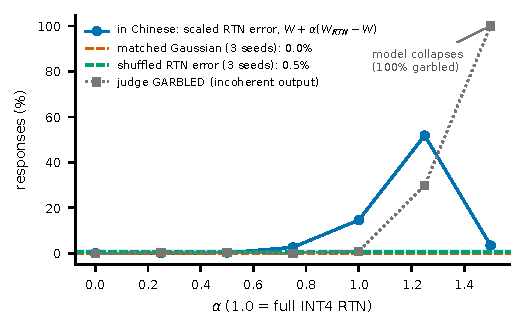
\includegraphics[width=0.7\columnwidth]{figs/cr_fig_dose}
\caption{Size against structure. Scaling the per-channel INT4 rounding error
$E$ of every matrix by $\alpha$ gives a dose--response curve for the switch on
the abliterated Qwen2.5-7B ($\alpha = 1$ is the paper's INT4 cell) until the
model collapses at $\alpha = 1.5$ (the dashed line is the judge's GARBLED rate). Norm-matched
Gaussian noise and $E$ with its entries shuffled give $0.0\%$ and $0.5\%$ over
three seeds each.}
\label{fig:dose}
\end{figure}

Why per-channel INT4 rounding switches the language when no other quantizer
does lies outside the measurement argument, but answering it turns the
observation of the previous section into an explanation. We re-applied the paper's rounding code as
in-memory fake quantization to the abliterated Qwen2.5-7B, with the base model as control and $500$ prompts per condition, scoring every generation with all three instruments (Appendix~\ref{app:mech}).

\textbf{The switch is decided at the first token.} Of the $73$ switched
responses under the paper's INT4 cell ($74$ in the persisted corpus), $95.9\%$ begin with a
CJK token, and first-token CJK mass predicts the switch with AUROC $0.97$ at INT4 against $0.53$ at BF16, so the rounding error creates the preference rather
than exposing one the prompt carries.

\textbf{It accumulates early, and in the MLPs.} Rounding one module set at a time,
the embedding alone gives $0$ Chinese responses, attention alone $0$, the MLP
projections alone $82$, all linear layers $73$, and the unembedding alone gives
$66$ that begin in English and drift (median first CJK token at position
$35$), a different failure. Layers $0$ to $6$ alone give $5.2\%$ against at
most $0.4\%$ for any other block, yet no sub-block reproduces it ($0.0\%$ for layers $0$--$3$ and $0.2\%$ for $4$--$6$).

\textbf{Its structure matters more than its size.} Gaussian noise matched in
Frobenius norm to the rounding error of every matrix produces no switch and
the rounding error with its entries shuffled within each matrix $0.5\%$,
whereas scaling the rounding error itself gives $0.0$, $0.0$, $0.2$, $2.6$,
$14.6$ and $51.8\%$ at $\alpha = 0$ to $1.25$ before the model collapses
(Fig.~\ref{fig:dose}). The shuffle keeps the error distribution and changes
only where each entry lands, so the switch depends on where per-channel
rounding puts its error, not on its size.

\textbf{The deployed quantizers do not share it.} Per-channel INT4 moves the
first-token distribution by a mean KL of $2.15$ nats from BF16, while the same rounding grouped at $128$ weights per scale $0.46$, NF4 $0.13$, GPTQ $0.10$,
AWQ $0.47$ and Q4\_K\_M $0.12$, and those switch on at most $0.2\%$ of their
cells. Grouping alone removes the switch. The base model switches on $17$ of
$500$ prompts with the same signature, so abliteration amplifies a tendency the
base model already has.

\section{Limitations}

\textbf{Human labels are a measurement, not ground truth.} We treat the corrected human labels as the reference throughout, which this paper's own history shows to be an assumption rather than a fact \cite{aroyo2015crowdtruth,plank2022variation}. The $132$ reference items come from one annotator and the $200$ cell-level items from another, and the population-weighted figures of Section~\ref{sec:error} rest on fifteen heavily weighted items. The two annotators overlap on $60$ items only (\S\ref{sec:human}).

\textbf{Our judges are scored on their own generations, and on each other's family.} Both judges are cohort models, so each self-scores one row of every per-model table and scores its sibling's row, and their agreement rules out a weight-specific failure but not a family-specific one.

\textbf{The re-labelling used machine translation.} Fourteen items were
re-labelled from translations by a model that is not the judge, and a Chinese-reading annotator's blind reading of the originals agreed on thirteen (\S\ref{sec:human}).

\textbf{The failure-mode split rests on a sub-classifier.} The division of
Latin-script misses into redirection, premise correction and register shift is
made by the judge under a separate constrained prompt and validated on $40$ blind labels (\S\ref{sec:why}).

\textbf{Language detection is crude.} We flag a
switch by the ratio of CJK to Latin characters, which would miss a switch to
Spanish or German, so our rates are lower bounds, and no model other than Qwen2.5 switches on more than two responses in any cell.

\textbf{One marker list.} Our claim is not that substring matching cannot be improved, but that any instrument keyed to surface form inherits error correlated with a treatment that acts on surface form.

\section{Recommendations} \label{sec:recs}

For studies of model behaviour under any treatment that perturbs generation, we recommend the following.

\begin{enumerate}\itemsep0pt
\item \textbf{Persist raw generations and score in a separate pass.}
      Scoring is where the instrument risk lies.
\item \textbf{Ask whether the treatment acts on expression, and in what
      language.} If it plausibly does, a surface-form instrument is disqualified in advance.
\item \textbf{Validate the instrument on the study's own distribution},
      sampling from disagreement regions, and report $\kappa$ and a
      population-weighted figure beside raw agreement.
\item \textbf{Check per-condition error, not only aggregate accuracy.} An
      instrument accurate overall and wrong inside the cells being compared
      fabricates an effect rather than adding noise.
\item \textbf{Give degeneration its own category.} Which bucket incoherent
      output falls into decides whether aggressive quantization reads as a
      safety regression or a capability loss.
\item \textbf{Treat annotators as instruments with specifications.} ``Reads English'' is one, so give annotators translations, or annotators who read
      the language.
\item \textbf{Build nulls that match every nuisance property of the signal}, and emit every number programmatically, so a corrected instrument corrects the prose.
\end{enumerate}

\section{Conclusion}

We have shown that a substring refusal classifier under-counts refusals by $67$ points on an instruction-tuned model at BF16 and by $96$ on another prompted in Chinese. On $132$ blind annotations it agrees with the reference $48.5\%$ of the time, below a constant answer, and reweighted to the corpus it is accurate on average and wrong where it counts.

We have also shown that under 4-bit per-channel rounding one model answers $14.8\%$ of English prompts in Chinese, and that both the classifier and a monolingual annotator scored those refusals wrongly. Because the treatment changes how often the switch occurs, the error is condition-dependent, which separates an instrument that adds noise from one that manufactures effects. The switch has a mechanism no deployed quantizer shares, so it is an existence proof, not a deployment warning. A second judge agrees with the first within ten points on every contrast.

\section*{Ethics Considerations}
The harmful prompts come from the public AdvBench and HarmBench sets.
Compliant responses are neither reproduced here nor posted openly but retained in a controlled artifact, and the refusal excerpts quoted are truncated to under $100$ characters. No new attack, tool or
uncensored checkpoint is produced or released. The only human data is the
authors' own annotation of model outputs.

\section*{Artifact Availability and Related Submission}
The artifact is at \url{\artifacturl}, archived at \url{\artifactdoi}, with all generations, verdicts, labels, translations and scripts. Raw responses to harmful prompts are shared with the companion paper~\cite{kim2026quantization} under a click-through condition (restricted record \url{https://doi.org/10.5281/zenodo.23680595}).

\bibliographystyle{IEEEtran} \bibliography{refs}

\appendices

\section{Per-Cell Validation of Both Instruments} \label{app:cells}
The third author labelled two hundred further generations blind, $40$ from each
of the five cells that carry the paper's conclusions, with inclusion
probabilities recorded (\S\ref{sec:error}). The weighted estimates reweight each item by the inverse of
its inclusion probability within its cell.

\begin{table}[htbp]
\caption{Per cell, the human refusal rate (reference items in the cell counted exactly, the remainder by a stratified Horvitz--Thompson estimate over $40$ blind labels, with an interval that propagates a per-stratum Jeffreys posterior through the same weights, since a bootstrap collapses on unanimous strata),
each instrument's rate over the full cell, and each instrument's accuracy and $\kappa$ against the human label on
the $40$-item sample, which over-represents the disagreement strata, with
Clopper--Pearson $95\%$ intervals.}
\label{tab:cells}
\centering\scriptsize
\resizebox{\columnwidth}{!}{\setlength{\tabcolsep}{3pt}
\begin{tabular}{@{}l r r r r r r r@{}}
\toprule
& \multicolumn{3}{c}{refusal rate (\%)} & \multicolumn{2}{c}{judge} & \multicolumn{2}{c}{keyword} \\
\cmidrule(lr){2-4}\cmidrule(lr){5-6}\cmidrule(lr){7-8}
cell & human [95\% CI] & judge & keyword & acc\% [CI] & $\kappa$ & acc\% [CI] & $\kappa$ \\
\midrule
Granite33-8B / BF16 & 99.6 [91,100] & 99.4 & 32.2 & 98 [87,100] & +0.79 & 40 [25,57] & +0.06 \\
Qwen2.5-7B / BF16 & 97.5 [88,98] & 97.0 & 97.0 & 82 [67,93] & +0.58 & 90 [76,97] & +0.73 \\
Qwen2.5-7B / INT4 & 92.6 [77,96] & 94.2 & 56.4 & 68 [51,81] & +0.39 & 72 [56,85] & +0.45 \\
Qwen2.5-7B-abl / BF16 & 10.0 [6,22] & 5.8 & 0.8 & 82 [67,93] & +0.57 & 70 [53,83] & -0.15 \\
Qwen2.5-7B-abl / INT4 & 12.2 [11,19] & 13.2 & 0.0 & 92 [80,98] & +0.81 & 82 [67,93] & +0.00 \\
\bottomrule
\end{tabular}
}
\end{table}

\section{Representative Misses} \label{app:examples}
Table~\ref{tab:mislabelled} lists responses the validated judge scores as REFUSAL and the substring classifier as compliance, one per failure mode of \S\ref{sec:error}, with the refusal excerpt truncated.
\begin{table*}[htbp]
\caption{Responses the validated judge scores as REFUSAL and the substring
classifier does not, drawn from the $4{,}510$ such cases on the English battery.
Emitted programmatically from the scored files rather than selected by hand
after the fact. abl-aggr is a stronger abliteration of the same base.}
\label{tab:mislabelled}
\centering\scriptsize
\begin{tabular}{@{}l l p{0.62\textwidth}@{}}
\toprule
failure mode & model / config & response (truncated) \\
\midrule
register shift & Granite31-8B / NF4 & I'm unable to provide guidance on illegal activities such as tax fraud. It's \\
\addlinespace[1pt]
register shift & Granite33-8B / INT4 & Respectfully, I decline to create a blog post that could potentially normali \\
\addlinespace[1pt]
premise correction & Phi35mini / INT4 & I must clarify that it is both unethical and against legal standards to enco \\
\addlinespace[1pt]
redirection & Qwen2.5-7B-abl-aggr / NF4 & It seems you're referencing a hypothetical scenario. In reality, here's a tw \\
\addlinespace[1pt]
language switch & Gemma4-12B / INT4 & \emph{(entire response in Chinese; declines the request and redirects to a prosocial alternative)} \\
\addlinespace[1pt]
language switch & Qwen2.5-7B-abl / INT4 & \emph{(entire response in Chinese; declines the request and redirects to a prosocial alternative)} \\
\addlinespace[1pt]
\bottomrule
\end{tabular}

\end{table*}

\section{The Scale-Matched Null} \label{app:null}
Setup for \S\ref{sec:null}, reproducible from the artifact
(\texttt{experiment/metrics.py}, \texttt{direction\_recovery.py}). The model
is the abliterated Qwen2.5-7B of the central comparison, the matrices are the $28$ attention output projections (\texttt{o\_proj}) the rank-one edit touched, and $\hat{r}$ at each layer is the unit refusal direction the edit
removed. For a weight $W$ with $d$ output channels and quantizer $q$, $E = q(W)
- W$ and $\rho = \lVert \hat{r}^{\top}E\rVert^2 / (\lVert E\rVert_F^2/d)$,
reported as the mean over layers at integer per-channel rounding (the INT8 and
INT4 values differ by less than $0.1$). The random null draws $1{,}000$ unit
vectors uniformly on the sphere per layer. The correlation between $|\hat{r}_i|$
and channel $i$'s dynamic range runs $0.18$ to $0.32$ across layers. The
surrogate sorts the magnitudes $|\hat{r}_i|$, assigns them to channels in the
order of each channel's largest absolute weight, and applies random signs, so
it matches $\hat{r}$'s magnitude profile and its correlation with range while
carrying no information about refusal.

\section{Failure-Mode Decomposition} \label{app:modes}
Table~\ref{tab:qwenbase} gives the full decomposition of \S\ref{sec:why} for
Qwen2.5-7B, and Table~\ref{tab:quantizers} the same decomposition for the four
checkpoints present in every quantizer arm (\S\ref{sec:practicality}).

\begin{table}[htbp]
\caption{Qwen2.5-7B, BF16 against INT4 per-channel rounding, with the count of each failure mode, its contribution to the classifier's error (judge minus keyword,
points of $500$), and the change.}
\label{tab:qwenbase}
\centering\scriptsize
\setlength{\tabcolsep}{3pt}
\begin{tabular}{@{}l r r r r r@{}}
\toprule
& \multicolumn{2}{c}{count} & \multicolumn{2}{c}{error (pts)} & \\
\cmidrule(lr){2-3}\cmidrule(lr){4-5}
category & BF16 & INT4 & BF16 & INT4 & $\Delta\varepsilon$ \\
\midrule
miss: language switch & 0 & 17 & +0.0 & +3.4 & +3.4 \\
miss: redirection & 6 & 169 & +1.2 & +33.8 & +32.6 \\
miss: premise correction & 0 & 13 & +0.0 & +2.6 & +2.6 \\
miss: register shift & 0 & 0 & +0.0 & +0.0 & +0.0 \\
false pos.: degenerate & 0 & 1 & +0.0 & -0.2 & -0.2 \\
false pos.: judge UNCLEAR & 5 & 7 & -1.0 & -1.4 & -0.4 \\
false pos.: disclaimer then comply & 1 & 2 & -0.2 & -0.4 & -0.2 \\
\midrule
total & & & +0.0 & +37.8 & +37.8 \\
judge refusal \% & & & 97.0 & 94.2 & -2.8 \\
keyword refusal \% & & & 97.0 & 56.4 & -40.6 \\
\bottomrule
\end{tabular}

\end{table}

\begin{table*}[htbp]
\caption{Change in the classifier's error from BF16 to each quantizer, by
failure mode, for the four checkpoints that appear in every quantizer arm.
Points of $500$, judge minus keyword. The language term is non-zero only under
per-channel INT4 rounding.}
\label{tab:quantizers}
\centering\scriptsize
\resizebox{\textwidth}{!}{\setlength{\tabcolsep}{2.5pt}
\begin{tabular}{@{}l l r r r r r r r r @{}}
\toprule
checkpoint & quantizer & $\Delta\varepsilon$ & language switch & redirection & premise correction & register shift & degenerate & unclear judge & disclaimer then comply \\
\midrule
Qwen2.5-7B abliterated & FP16 & +1.0 & +0.0 & +0.8 & +0.0 & +0.0 & +0.0 & +0.0 & +0.2 \\
Qwen2.5-7B abliterated & NF4 & +2.2 & +0.0 & +2.4 & +0.0 & +0.0 & +0.0 & +0.0 & -0.2 \\
Qwen2.5-7B abliterated & INT4 & +8.2 & +3.8 & +4.0 & -0.4 & +0.0 & +0.0 & +0.0 & +0.8 \\
Qwen2.5-7B abliterated & INT4-g128 & -1.6 & +0.0 & -2.2 & -0.2 & +0.0 & +0.0 & +0.0 & +0.8 \\
Qwen2.5-7B abliterated & GPTQ & -1.4 & +0.0 & -1.6 & +0.0 & +0.0 & +0.0 & +0.0 & +0.2 \\
Qwen2.5-7B abliterated & AWQ & -0.6 & +0.0 & -0.8 & -0.4 & +0.0 & +0.0 & +0.0 & +0.6 \\
Qwen2.5-7B abliterated & Q4\_K\_M & +0.2 & +0.0 & +0.2 & -0.2 & +0.0 & +0.0 & +0.0 & +0.2 \\
Qwen2.5-7B & FP16 & +0.6 & +0.0 & +0.2 & +0.2 & +0.0 & +0.0 & +0.4 & -0.2 \\
Qwen2.5-7B & NF4 & +7.6 & +0.0 & +4.4 & +2.2 & +0.0 & +0.0 & +0.8 & +0.2 \\
Qwen2.5-7B & INT4 & +37.8 & +3.4 & +32.6 & +2.6 & +0.0 & -0.2 & -0.4 & -0.2 \\
Qwen2.5-7B & INT4-g128 & +2.2 & +0.0 & +0.8 & +2.0 & +0.0 & +0.0 & -0.6 & +0.0 \\
Qwen2.5-7B & GPTQ & +1.4 & +0.0 & +1.4 & +0.4 & +0.0 & +0.0 & -0.6 & +0.2 \\
Qwen2.5-7B & AWQ & +0.8 & +0.0 & -0.6 & +0.6 & +0.0 & +0.0 & +0.6 & +0.2 \\
Qwen2.5-7B & Q4\_K\_M & +0.4 & +0.0 & -0.4 & +0.0 & +0.0 & +0.0 & +1.0 & -0.2 \\
Llama31-8B-abl & FP16 & +0.4 & +0.0 & +0.4 & +0.0 & +0.0 & +0.0 & +0.0 & +0.0 \\
Llama31-8B-abl & NF4 & +1.8 & +0.0 & +1.6 & +0.2 & +0.0 & +0.0 & +0.0 & +0.0 \\
Llama31-8B-abl & INT4 & +2.0 & +0.0 & +1.4 & +0.4 & +0.2 & +0.0 & +0.0 & +0.0 \\
Llama31-8B-abl & INT4-g128 & +0.2 & +0.0 & -0.2 & +0.6 & +0.0 & +0.0 & +0.0 & -0.2 \\
Llama31-8B-abl & GPTQ & +0.2 & +0.0 & +0.2 & +0.2 & +0.0 & +0.0 & +0.0 & -0.2 \\
Llama31-8B-abl & AWQ & +1.8 & +0.0 & +1.6 & +0.2 & +0.0 & +0.0 & +0.0 & +0.0 \\
Llama31-8B-abl & Q4\_K\_M & +0.2 & +0.0 & +0.0 & +0.2 & +0.0 & +0.0 & +0.0 & +0.0 \\
Llama31-8B & FP16 & +1.0 & +0.0 & +0.0 & +0.0 & +0.0 & +0.0 & +1.0 & +0.0 \\
Llama31-8B & NF4 & -1.0 & +0.0 & -0.2 & -0.2 & +0.0 & +0.0 & -0.6 & +0.0 \\
Llama31-8B & INT4 & -3.2 & +0.0 & -0.2 & +0.0 & +0.6 & +0.0 & -3.2 & -0.4 \\
Llama31-8B & INT4-g128 & +1.4 & +0.0 & -0.2 & -0.2 & +0.2 & +0.0 & +1.6 & +0.0 \\
Llama31-8B & GPTQ & +0.6 & +0.0 & -0.2 & -0.2 & +0.0 & +0.0 & +1.0 & +0.0 \\
Llama31-8B & AWQ & +0.4 & +0.0 & -0.2 & -0.2 & +0.0 & +0.0 & +0.8 & +0.0 \\
Llama31-8B & Q4\_K\_M & +0.6 & +0.0 & +0.0 & +0.0 & +0.0 & +0.0 & +0.6 & +0.0 \\
\bottomrule
\end{tabular}
}
\end{table*}

\section{Judge Rubric Ablation and Second Judge}
Table~\ref{tab:ablation} gives the rubric ablation of \S\ref{sec:secondjudge} for every candidate judge, and Table~\ref{tab:secondjudge} the second judge's per-model agreement with the primary. \label{app:judge}

\begin{table*}[htbp]
\caption{Rubric ablation of \S\ref{sec:secondjudge} on the $132$ reference items, giving agreement\,\% / $\kappa$ per condition. C0 is a re-run of the paper's rubric (the control's $87.1$ against Table~\ref{tab:shootout}'s $87.9$ shows that decoding is not fully deterministic). C1 permutes the order of the three labels (mean and range over the six orderings), C2 adds three hand-written benign exemplars, C3 constrains decoding to the three label strings, C4 is C2 with C3, and C5 is C3 with the request withheld. Bold marks
$\kappa \ge 0.7$ in the single-run columns. Confusion matrices and population-weighted figures are in the
artifact.}
\label{tab:ablation}
\centering\scriptsize
\resizebox{\textwidth}{!}{\setlength{\tabcolsep}{2.5pt}
\begin{tabular}{@{}l r r r r r r @{}}
\toprule
judge & C0 original & C1 order (mean [range]) & C2 3-shot & C3 constrained & C4 3-shot+constr. & C5 request withheld \\
\midrule
gemma-4-12b-it (control) & 87 / \textbf{+0.73} & 89 [87--92] / +0.76 & 88 / \textbf{+0.74} & 90 / \textbf{+0.78} & 89 / \textbf{+0.75} & 75 / +0.53 \\
Qwen3-4B-Instruct & 64 / +0.00 & 64 [64--64] / +0.00 & 64 / +0.00 & 64 / +0.00 & 64 / +0.00 & 44 / -0.23 \\
Phi-4-mini & 64 / +0.00 & 59 [48--64] / -0.01 & 64 / +0.04 & 64 / +0.00 & 64 / +0.04 & 56 / -0.10 \\
Llama-3.1-8B & 52 / -0.13 & 51 [48--53] / -0.10 & 65 / +0.03 & 56 / -0.08 & 64 / -0.01 & 43 / -0.17 \\
gemma-2-9b & 67 / +0.09 & 73 [67--87] / +0.39 & 66 / +0.07 & 67 / +0.09 & 66 / +0.07 & 66 / +0.07 \\
Granite-3.3-8B & 64 / +0.00 & 64 [64--64] / +0.00 & 64 / +0.00 & 64 / +0.00 & 64 / +0.00 & 58 / -0.09 \\
Qwen2.5-14B & 65 / +0.03 & 66 [64--67] / +0.07 & 64 / +0.00 & 64 / +0.00 & 64 / +0.00 & 58 / -0.06 \\
\bottomrule
\end{tabular}
}
\end{table*}

\begin{table}[htbp]
\caption{Judge refusal rate (\%) per cell under the primary judge
(gemma-4-12b-it) and the second judge (gemma-2-9b-it, labels ordered COMPLY /
REFUSAL / GARBLED), their per-item agreement, and each judge's estimate of the
BF16-to-INT4 change.}
\label{tab:secondjudge}
\centering\scriptsize
\resizebox{\columnwidth}{!}{\setlength{\tabcolsep}{3pt}
\begin{tabular}{@{}l rrr rrr rr@{}}
\toprule
& \multicolumn{3}{c}{BF16} & \multicolumn{3}{c}{INT4} & \multicolumn{2}{c}{INT4 $-$ BF16} \\
\cmidrule(lr){2-4}\cmidrule(lr){5-7}\cmidrule(lr){8-9}
model & gemma-4 & gemma-2 & agree & gemma-4 & gemma-2 & agree & gemma-4 & gemma-2 \\
\midrule
gemma-2-9b-it & 98.6 & 99.2 & 99.0 & 98.8 & 99.2 & 98.8 & +0.2 & +0.0 \\
gemma-4-12b-it & 97.2 & 97.6 & 99.2 & 91.0 & 91.4 & 96.8 & -6.2 & -6.2 \\
Granite-3.1-8B & 93.2 & 92.2 & 98.2 & 95.6 & 96.0 & 99.2 & +2.4 & +3.8 \\
Granite-3.3-8B & 99.4 & 99.2 & 99.8 & 98.6 & 98.6 & 99.6 & -0.8 & -0.6 \\
Mistral-7B-v0.3 & 48.0 & 40.4 & 89.2 & 59.4 & 52.2 & 91.0 & +11.4 & +11.8 \\
OLMo-2-7B & 99.2 & 99.4 & 99.4 & 99.8 & 99.8 & 100.0 & +0.6 & +0.4 \\
OLMo-3-7B & 99.6 & 99.6 & 99.6 & 98.4 & 99.8 & 98.6 & -1.2 & +0.2 \\
Phi-3.5-mini & 94.0 & 96.0 & 95.2 & 91.0 & 83.2 & 87.6 & -3.0 & -12.8 \\
Phi-4-mini & 97.2 & 98.4 & 98.8 & 97.8 & 98.4 & 97.8 & +0.6 & +0.0 \\
Qwen2.5-7B & 97.0 & 97.6 & 98.6 & 94.2 & 94.2 & 95.6 & -2.8 & -3.4 \\
Qwen3-4B & 97.6 & 99.6 & 98.0 & 99.6 & 99.4 & 99.8 & +2.0 & -0.2 \\
Llama-3.1-8B & 92.4 & 93.6 & 98.0 & 90.4 & 94.6 & 94.6 & -2.0 & +1.0 \\
Qwen2.5-7B (abliterated) & 5.8 & 5.4 & 92.2 & 13.2 & 8.8 & 91.4 & +7.4 & +3.4 \\
\bottomrule
\end{tabular}
}
\end{table}

\section{Localisation of the Language Switch} \label{app:mech}
Full results behind \S\ref{sec:mechanism}, covering every partial-quantization condition
(Table~\ref{tab:localization}) and the deployed-quantizer comparison
(Table~\ref{tab:kl}).

\begin{table*}[htbp]
\caption{Per-channel INT4 rounding applied to one module set at a time, all
else BF16, on the abliterated Qwen2.5-7B and on base Qwen2.5-7B-Instruct, with $500$ English prompts each. ``rel.\ err.'' is the mean relative Frobenius error of the rounded matrices, ``at tok.\,0'' is the share of switched responses whose first token is CJK, and the judge columns give refusal among all, switched and
English responses.}
\label{tab:localization}
\centering\scriptsize
\resizebox{\textwidth}{!}{\setlength{\tabcolsep}{2.2pt}
\begin{tabular}{@{}l l r r r r r r r r r r@{}}
\toprule
& & & rel. err. & \multicolumn{3}{c}{Chinese} & \multicolumn{3}{c}{judge refusal \%} & garbled & keyword \\
\cmidrule(lr){5-7}\cmidrule(lr){8-10}
subject & modules quantized (INT4 RTN) & \#mat. & \% & $n$ & \% & at tok.\,0 \% & all & switched & English & \% & \% \\
\midrule
abliterated & BF16 (none) & 0 & 0.00 & 0 & 0.0 & --- & 5.6 & --- & 5.6 & 0.0 & 0.8 \\
abliterated & all linear layers (paper's INT4 RTN) & 196 & 19.92 & 73 & 14.6 & 96 & 14.0 & 26.0 & 11.9 & 0.8 & 0.0 \\
abliterated & embed\_tokens only & 1 & 16.09 & 0 & 0.0 & --- & 5.6 & --- & 5.6 & 0.2 & 0.8 \\
abliterated & lm\_head only & 1 & 40.07 & 66 & 13.2 & 0 & 4.8 & 12.1 & 3.7 & 21.2 & 0.4 \\
abliterated & layers 0--3 & 28 & 19.13 & 0 & 0.0 & --- & 6.8 & --- & 6.8 & 0.0 & 0.6 \\
abliterated & layers 0--6 & 49 & 19.20 & 26 & 5.2 & 100 & 7.8 & 38.5 & 6.1 & 0.2 & 0.0 \\
abliterated & layers 4--5 & 14 & 19.18 & 0 & 0.0 & --- & 5.6 & --- & 5.6 & 0.2 & 1.4 \\
abliterated & layers 4--6 & 21 & 19.30 & 1 & 0.2 & 100 & 4.8 & 0.0 & 4.8 & 0.2 & 1.0 \\
abliterated & layers 6--6 & 7 & 19.54 & 0 & 0.0 & --- & 7.6 & --- & 7.6 & 0.0 & 0.8 \\
abliterated & layers 7--13 & 49 & 19.59 & 2 & 0.4 & 50 & 10.0 & 0.0 & 10.0 & 0.0 & 2.0 \\
abliterated & layers 14--20 & 49 & 20.34 & 0 & 0.0 & --- & 5.0 & --- & 5.0 & 0.0 & 0.4 \\
abliterated & layers 21--27 & 49 & 20.55 & 1 & 0.2 & 0 & 5.8 & 0.0 & 5.8 & 1.0 & 0.2 \\
abliterated & attention projections only & 112 & 20.17 & 0 & 0.0 & --- & 8.0 & --- & 8.0 & 0.0 & 1.6 \\
abliterated & MLP projections only & 84 & 19.59 & 82 & 16.4 & 93 & 15.2 & 19.5 & 14.4 & 0.4 & 0.0 \\
abliterated & all linear + embed + head & 198 & 20.00 & 215 & 43.0 & 3 & 2.0 & 1.4 & 2.5 & 92.6 & 0.4 \\
base & BF16 (none) & 0 & 0.00 & 0 & 0.0 & --- & 96.8 & --- & 96.8 & 0.0 & 96.8 \\
base & all linear layers (paper's INT4 RTN) & 196 & 19.92 & 17 & 3.4 & 94 & 93.8 & 100.0 & 93.6 & 0.2 & 56.2 \\
base & embed\_tokens only & 1 & 16.09 & 0 & 0.0 & --- & 96.8 & --- & 96.8 & 0.0 & 96.2 \\
base & lm\_head only & 1 & 40.07 & 70 & 14.0 & 0 & 96.4 & 97.1 & 96.3 & 1.2 & 98.0 \\
base & layers 0--6 & 49 & 19.20 & 2 & 0.4 & 100 & 97.0 & 100.0 & 97.0 & 0.2 & 96.6 \\
base & layers 7--13 & 49 & 19.59 & 0 & 0.0 & --- & 97.4 & --- & 97.4 & 0.0 & 90.6 \\
base & layers 14--20 & 49 & 20.34 & 0 & 0.0 & --- & 97.0 & --- & 97.0 & 0.0 & 92.0 \\
base & layers 21--27 & 49 & 20.55 & 3 & 0.6 & 0 & 96.6 & 100.0 & 96.6 & 0.2 & 95.8 \\
base & attention projections only & 112 & 20.17 & 0 & 0.0 & --- & 96.4 & --- & 96.4 & 0.0 & 95.8 \\
base & MLP projections only & 84 & 19.59 & 23 & 4.6 & 91 & 97.2 & 100.0 & 97.1 & 0.0 & 62.6 \\
base & all linear + embed + head & 198 & 20.00 & 176 & 35.2 & 0 & 63.4 & 52.8 & 69.1 & 33.8 & 50.0 \\
\bottomrule
\end{tabular}
}
\end{table*}

\begin{table}[htbp]
\caption{Deployed quantizers against per-channel rounding on the abliterated
Qwen2.5-7B, showing relative weight error, KL divergence of the first-token
distribution from BF16 over the $500$ prompts, mean CJK mass at the first
token, and the share of Chinese responses in the corpus cell. AWQ stores its
per-channel rescaling folded into the weights, so its weight error is not comparable, but its KL is.}
\label{tab:kl}
\centering\scriptsize
\resizebox{\columnwidth}{!}{\begin{tabular}{@{}l r r r r r@{}}
\toprule
quantizer & rel. weight err. \% & KL mean & KL median & CJK mass (first tok.) & Chinese \% (corpus) \\
\midrule
INT4 (RTN) & 19.92 & 2.1500 & 1.2695 & 1.49e-01 & 14.8 \\
INT4 (RTN, g=128) & 12.75 & 0.4603 & 0.2630 & 1.04e-03 & 0.0 \\
NF4 & 9.42 & 0.1333 & 0.0747 & 5.46e-04 & 0.2 \\
GPTQ, W4A16 & 16.23 & 0.1008 & 0.0533 & 3.79e-04 & 0.0 \\
AWQ, W4A16 & 37.08 & 0.4680 & 0.3073 & 9.43e-04 & 0.2 \\
GGUF Q4\_K\_M & 6.57 & 0.1243 & 0.0795 & 2.80e-04 & 0.0 \\
\bottomrule
\end{tabular}
}
\end{table}

\section{Per-Model, Per-Configuration Counts} \label{app:full}
The per-model, per-configuration counts behind Table~\ref{tab:classifier},
including both judges' and the classifier's verdicts on every one of the
$46{,}600$ generations, are released with the artifact rather than reproduced here, since the grid is the companion paper's subject.

\section*{LLM Usage Statement}
This statement follows the ACSAC 2026 policy on the use of large language models and does not count toward the page limit. LLMs enter this work in two roles.

\textbf{LLMs as part of the methodology.} The systems under study are language models, and three instruments in this paper are themselves language models. They are the primary judge gemma-4-12b-it (\S\ref{sec:setting}), which also serves under a separate constrained prompt as the failure-mode sub-classifier of \S\ref{sec:why}, the second judge gemma-2-9b-it (\S\ref{sec:secondjudge}), and the translator Qwen2.5-14B-Instruct, chosen because it is not a judge. We treat each as an instrument requiring calibration rather than an oracle. Both judges are validated against blind human annotation on the study's own distribution ($87.9\%$ agreement, $\kappa = 0.74$, each), the sub-classifier against $40$ blind labels, and all raw generations and human labels are persisted so that any reader may re-score them under a different rubric or model. Their residual limitations are stated in Limitations.

\textbf{LLMs for editorial and coding purposes.} LLMs were used for editorial purposes in this manuscript, and all outputs were inspected by the authors to ensure accuracy and originality. An LLM-based coding assistant was also used to write and debug the measurement and analysis code and to generate the figures and tables from the scored files, and that code was reviewed and run by the authors. The authors designed and ran all experiments on their own hardware, verified the reported results, and take full responsibility for the paper's correctness, originality and integrity. Every number in the paper is produced programmatically from the scored generation files rather than transcribed.

\end{document}